%%%%%%%%%%%%%%%%%%%%%%%%%%%%%%%%%%%%%%%
%
% Using Diaz essay LaTeX template from:
% http://www.LaTeXTemplates.com
%
% Authors:
% Vel (vel@LaTeXTemplates.com)
% Nicolas Diaz (nsdiaz@uc.cl)
%
% License:
% CC BY-NC-SA 3.0 (http://creativecommons.org/licenses/by-nc-sa/3.0/)
%
%%%%%%%%%%%%%%%%%%%%%%%%%%%%%%%%%%%%%%%%%

% PACKAGES AND OTHER DOCUMENT CONFIGURATIONS
\documentclass[11pt]{diazessay} % Font size (can be 10pt, 11pt or 12pt)

\usepackage{listings}
\usepackage{tikz}
\usepackage{hyperref}
\usetikzlibrary{positioning}
\usetikzlibrary{arrows}

\lstset{frame=tb,
  language=C,
  aboveskip=3mm,
  belowskip=3mm,
  showstringspaces=false,
  columns=flexible,
  basicstyle={\small\ttfamily},
  numbers=none,
  numberstyle=\tiny\color{gray},
  keywordstyle=\color{blue},
  commentstyle=\color{black},
  %stringstyle=\color{mauve},
  breaklines=false,
  breakatwhitespace=false,
  tabsize=3
}

% Defines a `datastore' shape for use in DFDs.  This inherits from a
% rectangle and only draws two horizontal lines.
\makeatletter
\pgfdeclareshape{datastore}{
  \inheritsavedanchors[from=rectangle]
  \inheritanchorborder[from=rectangle]
  \inheritanchor[from=rectangle]{center}
  \inheritanchor[from=rectangle]{base}
  \inheritanchor[from=rectangle]{north}
  \inheritanchor[from=rectangle]{north east}
  \inheritanchor[from=rectangle]{east}
  \inheritanchor[from=rectangle]{south east}
  \inheritanchor[from=rectangle]{south}
  \inheritanchor[from=rectangle]{south west}
  \inheritanchor[from=rectangle]{west}
  \inheritanchor[from=rectangle]{north west}
  \backgroundpath{
    %  store lower right in xa/ya and upper right in xb/yb
    \southwest \pgf@xa=\pgf@x \pgf@ya=\pgf@y
    \northeast \pgf@xb=\pgf@x \pgf@yb=\pgf@y
    \pgfpathmoveto{\pgfpoint{\pgf@xa}{\pgf@ya}}
    \pgfpathlineto{\pgfpoint{\pgf@xb}{\pgf@ya}}
    \pgfpathmoveto{\pgfpoint{\pgf@xa}{\pgf@yb}}
    \pgfpathlineto{\pgfpoint{\pgf@xb}{\pgf@yb}}
 }
}
\makeatother

% TITLE SECTION
\title{\textbf{How To Use Perf To Debug Perf}}
\author{\textbf{Leo Yan} \textit{<leo.yan@linaro.org>}} % Author and institution
\date{\today} % Date, use \date{} for no date

\def\code#1{\texttt{#1}}

%----------------------------------------------------------------------------------------

\begin{document}

\maketitle % Print the title section

% ABSTRACT AND KEYWORDS

\begin{abstract}
Debugging is for inspecting a program, for both user space and kernel space.
The perf tool contains complex logic for exchanging data through system calls,
making it a common practice to debug perf in everyday life.

This article explores various debugging techniques, organized from simple to
complex, with using the perf tool as the target program. As it explores these
debugging methods, the attention is directed towards the perf as debugging
tool. Ultimately, the article explains how to use perf to debug perf.
\end{abstract}

\hspace*{3.6mm}\textit{Keywords: Linux, debug, ftrace, kprobe, uprobe, perf } % Keywords
\vspace{30pt} % Vertical whitespace between the abstract and first section

% ESSAY BODY

\section*{Introduction}

First of all, this article has no plan to address traditional debuggers, e.g.
GDB or JTAG based debuggers. These tools use stop-the-world method to debug
programs: it firstly stops a target program, then it takes chance to check
the context for the program. The \textit{context} can be a software concept,
e.g. a thread or task context, a debugger can read variables from the task's
stack or heap. The \textit{context} can be a hardware context as well - when
a developer is using JTAG debugger to connect hardware and stop CPU, the
hardware registers and memory can be reviewed.

The purpose of this documentation is to discuss tools which can provide
tracing capability in runtime. The trace data is recorded in certain format
for afterwards analysis.

The content is divided into four sections:
\begin{itemize}
	\item Printing;
	\item Debugging with ftrace;
	\item Dynamic tracing;
	\item Using perf for debugging.
\end{itemize}

\section*{Printing}

Usually, a beginner studying C programming learns the first code piece is for
printing the string 'hello world!'.

\begin{lstlisting}
#include <stdio.h>
int main(void)
{
        printf("Hello World!\n");
        return 0;
}
\end{lstlisting}

The above code implicitly introduces a handy tracing tool: libc's
\code{printf()}. Then, when starting to access the Linux kernel, its
equivalent function \code{printk()} will no longer be strange.

A printing log means an event has occurred, alongside variables can be printed
out - this is perfect to act as tracing.

The printing is reliable in most cases. \code{printk()} is a context safe API
- even if a developer has no knowledge for interrupt context, thread context
and bottom-half context (e.g. in softirq or tasklet), printing still can work
as a main debugging method.

On the other hand, developers need to tolerate cons introduced by printing.
If logs are output into the UART console, developers suffer performance
penalty caused by the low speed of the UART port. In a worse case, the
printing can alter program flow and might lead to the timing issues hardly to
be reproduced.

It becomes challenging for using printing to debug a program which crosses
both user space and kernel space. The reason is \code{printf()} and
\code{printk()} store logs in separate buffers, leading to logs being output
in out-of-order without readable.

To resolve this issue, syslog is suggested. A program needs to use
\code{syslog()} to replace \code{printf()} for routing logs to syslog
service, all modules supporting syslog in system can output logs into a
central place. Unfortunately, syslog is not supported in every Linux system,
and many programs (including the perf) don't support syslog at all.

\subsection*{Debugging with ftrace}

If we are looking for a better debugging tool with lower performance penalties
and support for tracing in both user space and kernel space, ftrace appears as
a promising candidate.

Firstly, ftrace uses a ring buffer to store trace data, allowing users to save
the trace data into a file for testing and then perform post-analysis. This
approach enables ftrace to avoid the tracing latency caused by console, unlike
printing.

Secondly, ftrace supports both kernel and user space. The entire trace data is
recorded in a single file and displayed in a time-ordered format, thus the
output result is friendly for review.

\subsubsection*{Printing in ftrace}

Printing is supported in ftrace.

In the kernel, \code{trace\_printk()} is used to output logs into the ftrace
ring buffer. Once you use it, you will find this API quite useful: logs saved
in ftrace buffer will not be bothered by console's long latency, and by
enlarging buffer size, you will have sufficient capacity to store extensive
logs. These logs will not flood the console immediately, you can extract logs
into file whenever you want to parse them.

Ftrace provides a sysfs node called \code{trace\_marker} that allows the user
space to place logs into ftrace buffer. Through this interface, user space
events and kernel events can be synchronized together, thus developers can
understand a flow spanning the two spaces.

The kernel's documentation \code{Documentation/trace/ftrace.rst} gives an
example for how to write string into the \code{trace\_marker} node in C code:

\begin{lstlisting}
trace_fd = open("trace_marker", O_WRONLY);

void trace_write(const char *fmt, ...)
{
        va_list ap;
        char buf[256];
        int n;

        if (trace_fd < 0)
                return;

        va_start(ap, fmt);
        n = vsnprintf(buf, 256, fmt, ap);
        va_end(ap);

        write(trace_fd, buf, n);
}
\end{lstlisting}

A typical use case for \code{trace\_marker} is found in
\href{https://perfetto.dev/docs/data-sources/atrace}{ATrace}, which is a
part of Google's \href{https://ui.perfetto.dev/}{Perfetto} tool. Perfetto
is widely used for profiling Android UI performance and depends on the
ATrace to trace application events - the \code{trace\_marker} is the
underlying mechanism for tracing. While this article will remain on
fundamental debugging tools, it will not dive into ATrace's details.

\subsubsection*{Per CPU mode}

The option \code{--C} is used to collect samples only on the list of CPUs, the ring buffers are allocated for the specified CPUs.  For the example in figure 4, the perf command receives option \code{--C 0,2}, as the result, two ring buffers serve for CPU0 and CPU2 separately.

\begin{center}
\par
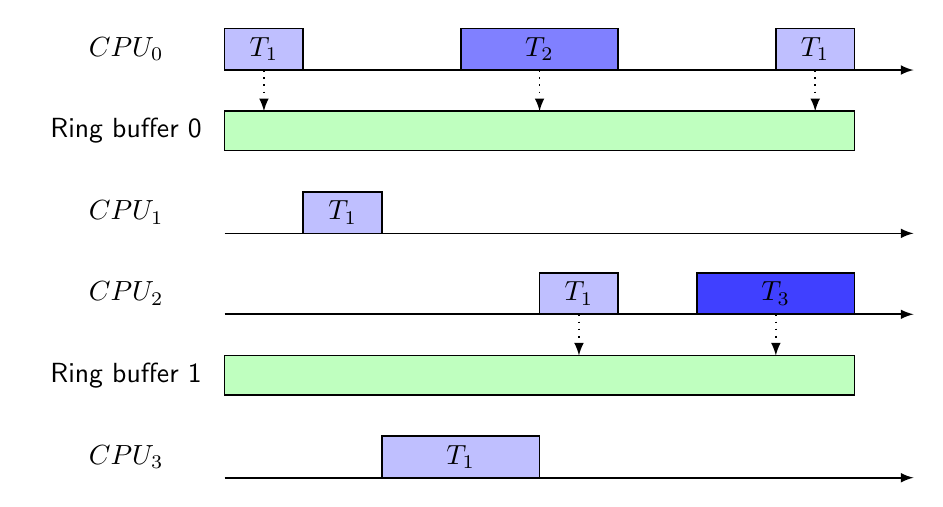
\begin{tikzpicture}[>=latex,font=\sffamily,semithick,scale=1.75]
	\node [minimum width=2.5cm,minimum height=.5cm,outer sep=0pt] at (0,0) (cpu0) {\( CPU_0 \)};
	\node [minimum width=1cm,minimum height=.5cm,outer sep=0pt,draw=black,fill=blue!25,right=0cm of cpu0] at (cpu0.east) (cpu0_p1_0) {\(T_{1}\)};
	\node [minimum width=2cm,minimum height=.5cm,outer sep=0pt,draw=black,fill=blue!50,right=3cm of cpu0] at (cpu0.east) (cpu0_p2_0) {\(T_{2}\)};
	\node [minimum width=1cm,minimum height=.5cm,outer sep=0pt,draw=black,fill=blue!25,right=7cm of cpu0] (cpu0_p1_1) {\(T_{1}\)};
	\draw[->] (cpu0.south east) -- +(5cm,0);

	\node [minimum width=2.5cm,minimum height=.5cm,outer sep=0pt,below=.5cm of cpu0] (rb0_txt) {Ring buffer 0};
	\node [minimum width=8cm,minimum height=.5cm,outer sep=0pt,draw=black,fill=green!25,right=0cm of rb0_txt] (rb0) {};

	\node [minimum width=2.5cm,minimum height=.5cm,outer sep=0pt,below=.5cm of rb0_txt] (cpu1) {\(CPU_{1}\)};
	\node [minimum width=1cm,minimum height=.5cm,outer sep=0pt,draw=black,fill=blue!25,right=1cm of cpu1] at (cpu1.east) (cpu1_p1_0) {\(T_{1}\)};
	\draw[->] (cpu1.south east) -- +(5cm,0);

	\node [minimum width=2.5cm,minimum height=.5cm,outer sep=0pt,below=.5cm of cpu1] (cpu2) {\(CPU_{2}\)};
	\node [minimum width=1cm,minimum height=.5cm,outer sep=0pt,draw=black,fill=blue!25,right=4cm of cpu2] (cpu2_p1_0) {\(T_{1}\)};
	\node [minimum width=2cm,minimum height=.5cm,outer sep=0pt,draw=black,fill=blue!75,right=6cm of cpu2] (cpu2_p3_0) {\(T_{3}\)};
	\draw[->] (cpu2.south east) -- +(5cm,0);

	\node [minimum width=2.5cm,minimum height=.5cm,outer sep=0pt,below=.5cm of cpu2] (rb1_txt) {Ring buffer 1};
	\node [minimum width=8cm,minimum height=.5cm,outer sep=0pt,draw=black,fill=green!25,right=0cm of rb1_txt] (rb1) {};

	\node [minimum width=2.5cm,minimum height=.5cm,outer sep=0pt,below=.5cm of rb1_txt] (cpu3) {\(CPU_{3}\)};
	\node [minimum width=2cm,minimum height=.5cm,outer sep=0pt,draw=black,fill=blue!25,right=2cm of cpu3] (cpu3_p1_0) {\(T_{1}\)};
	\draw[->] (cpu3.south east) -- +(5cm,0);


	\draw[->,dotted] (cpu0_p1_0.south) -- (cpu0_p1_0.south|-rb0.north);
	\draw[->,dotted] (cpu0_p1_1.south) -- (cpu0_p1_1.south|-rb0.north);
	\draw[->,dotted] (cpu0_p2_0.south) -- (cpu0_p2_0.south|-rb0.north);

	\draw[->,dotted] (cpu2_p1_0.south) -- (cpu2_p1_0.south|-rb1.north);
	\draw[->,dotted] (cpu2_p3_0.south) -- (cpu2_p3_0.south|-rb1.north);
\end{tikzpicture}
\par
\textbf{Figure 4: Ring buffer for per-cpu mode}
\end{center}

On the other hand, in this example even there have tasks running on CPU1 and CPU3, since the ring buffer is absent for these two CPUs, any activities on them will be ignored.

A usage case is to combine the options for per-thread mode and per-CPU mode, e.g. the option \code{--C 0,2 ----per--thread} is specified together; in this case, samples are recorded only when the profiled thread is scheduled on any of the listed CPUs.

\subsubsection*{System wide mode}

By default if without specifying mode, or explicitly using option \code{--a} or \code{----all--cpus}, perf collects samples on all CPUs, with the system wide mode.

In this mode, every CPU has its dedicated ring buffer; the interested events will be always enabled and sampled on every CPU, thus all threads are monitored, and the samples are recorded into the ring buffer belonging to the CPU which the events occurred on.

\begin{center}
\par
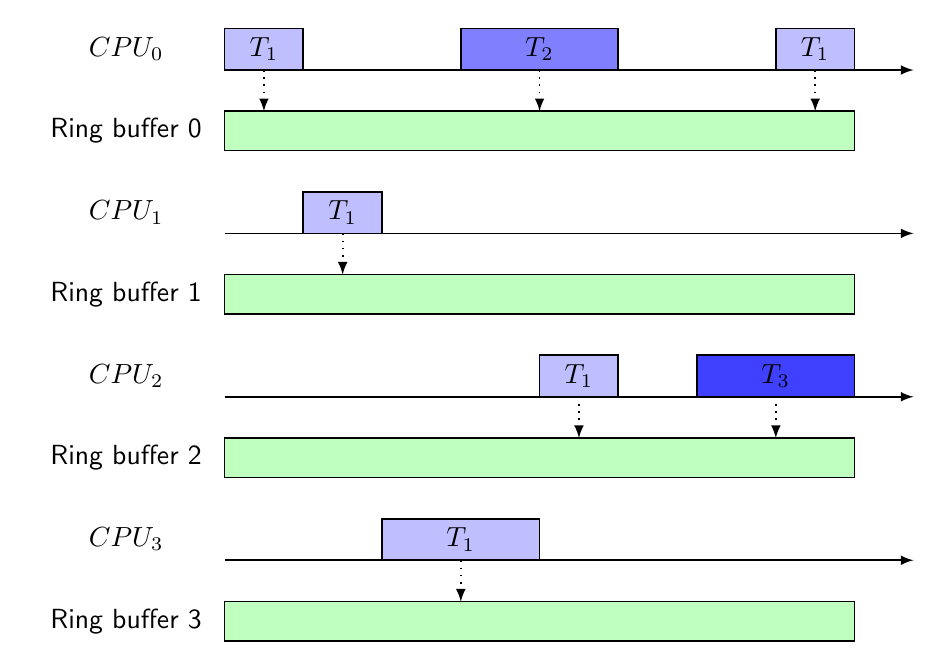
\begin{tikzpicture}[>=latex,font=\sffamily,semithick,scale=1.75]
	\node [minimum width=2.5cm,minimum height=.5cm,outer sep=0pt] at (0,0) (cpu0) {\( CPU_0 \)};
	\node [minimum width=1cm,minimum height=.5cm,outer sep=0pt,draw=black,fill=blue!25,right=0cm of cpu0] at (cpu0.east) (cpu0_p1_0) {\(T_{1}\)};
	\node [minimum width=2cm,minimum height=.5cm,outer sep=0pt,draw=black,fill=blue!50,right=3cm of cpu0] at (cpu0.east) (cpu0_p2_0) {\(T_{2}\)};
	\node [minimum width=1cm,minimum height=.5cm,outer sep=0pt,draw=black,fill=blue!25,right=7cm of cpu0] (cpu0_p1_1) {\(T_{1}\)};
	\draw[->] (cpu0.south east) -- +(5cm,0);

	\node [minimum width=2.5cm,minimum height=.5cm,outer sep=0pt,below=.5cm of cpu0] (rb0_txt) {Ring buffer 0};
	\node [minimum width=8cm,minimum height=.5cm,outer sep=0pt,draw=black,fill=green!25,right=0cm of rb0_txt] (rb0) {};

	\node [minimum width=2.5cm,minimum height=.5cm,outer sep=0pt,below=.5cm of rb0_txt] (cpu1) {\(CPU_{1}\)};
	\node [minimum width=1cm,minimum height=.5cm,outer sep=0pt,draw=black,fill=blue!25,right=1cm of cpu1] at (cpu1.east) (cpu1_p1_0) {\(T_{1}\)};
	\draw[->] (cpu1.south east) -- +(5cm,0);

	\node [minimum width=2.5cm,minimum height=.5cm,outer sep=0pt,below=.5cm of cpu1] (rb1_txt) {Ring buffer 1};
	\node [minimum width=8cm,minimum height=.5cm,outer sep=0pt,draw=black,fill=green!25,right=0cm of rb1_txt] (rb1) {};

	\node [minimum width=2.5cm,minimum height=.5cm,outer sep=0pt,below=.5cm of rb1_txt] (cpu2) {\(CPU_{2}\)};
	\node [minimum width=1cm,minimum height=.5cm,outer sep=0pt,draw=black,fill=blue!25,right=4cm of cpu2] (cpu2_p1_0) {\(T_{1}\)};
	\node [minimum width=2cm,minimum height=.5cm,outer sep=0pt,draw=black,fill=blue!75,right=6cm of cpu2] (cpu2_p3_0) {\(T_{3}\)};
	\draw[->] (cpu2.south east) -- +(5cm,0);

	\node [minimum width=2.5cm,minimum height=.5cm,outer sep=0pt,below=.5cm of cpu2] (rb2_txt) {Ring buffer 2};
	\node [minimum width=8cm,minimum height=.5cm,outer sep=0pt,draw=black,fill=green!25,right=0cm of rb2_txt] (rb2) {};

	\node [minimum width=2.5cm,minimum height=.5cm,outer sep=0pt,below=.5cm of rb2_txt] (cpu3) {\(CPU_{3}\)};
	\node [minimum width=2cm,minimum height=.5cm,outer sep=0pt,draw=black,fill=blue!25,right=2cm of cpu3] (cpu3_p1_0) {\(T_{1}\)};
	\draw[->] (cpu3.south east) -- +(5cm,0);

	\node [minimum width=2.5cm,minimum height=.5cm,outer sep=0pt,below=.5cm of cpu3] (rb3_txt) {Ring buffer 3};
	\node [minimum width=8cm,minimum height=.5cm,outer sep=0pt,draw=black,fill=green!25,right=0cm of rb3_txt] (rb3) {};

	\draw[->,dotted] (cpu0_p1_0.south) -- (cpu0_p1_0.south|-rb0.north);
	\draw[->,dotted] (cpu0_p1_1.south) -- (cpu0_p1_1.south|-rb0.north);
	\draw[->,dotted] (cpu0_p2_0.south) -- (cpu0_p2_0.south|-rb0.north);

	\draw[->,dotted] (cpu1_p1_0.south) -- (cpu1_p1_0.south|-rb1.north);

	\draw[->,dotted] (cpu2_p1_0.south) -- (cpu2_p1_0.south|-rb2.north);
	\draw[->,dotted] (cpu2_p3_0.south) -- (cpu2_p3_0.south|-rb2.north);

	\draw[->,dotted] (cpu3_p1_0.south) -- (cpu3_p1_0.south|-rb3.north);
\end{tikzpicture}
\par
\textbf{Figure 5: Ring buffer for system wide mode}
\end{center}

\subsection*{Writing and reading buffer}

From the previous section we get to know how the ring buffer is allocated for different modes, based on that this section will explain how the ring buffer is written or read.

\subsubsection*{Producer-consumer model}

It's a typical producer-consumer model for using the ring buffer.  In the Linux kernel, the events can produce samples which are stored into the ring buffer; the perf in user space consumes the samples by reading out the data from the ring buffer.

There have many occasions for generating samples: PMU interrupt handler when detecting event overflow, scheduling, dynamic tracepoint with kprobe/uprobe, static tracepoint, etc.  When a sample is recorded into the ring buffer, the kernel event core layer will wake up the thread which is polling on the events; perf works as a process to poll on the event, it will be waken up to read samples from the ring buffer.

\begin{center}
\par
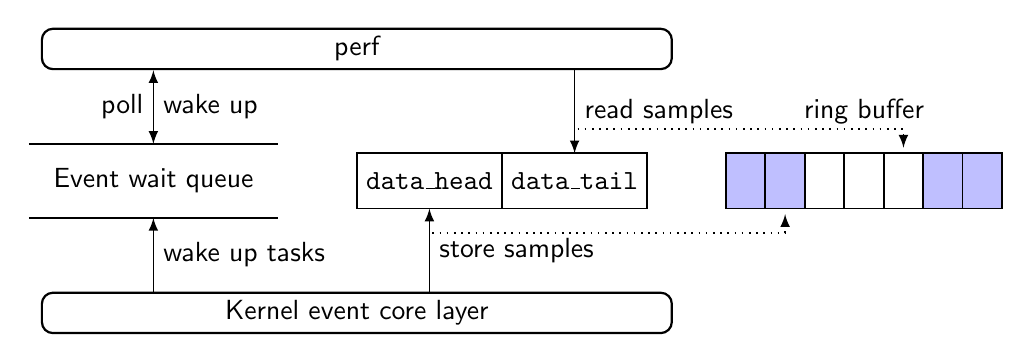
\begin{tikzpicture}[>=latex,font=\sffamily,semithick,scale=1.75]
	\node [minimum width=1cm,minimum height=2em,outer sep=0pt,draw=black,fill=white] at (0,0) (A) {\code{data\_head}};
	\node [minimum height=2em] at (A.east) (A2) {};
	\node [minimum width=1cm,minimum height=2em,outer sep=0pt,draw=black,fill=white,anchor=west] at (A.east) (B) {\code{data\_tail}};
        \node [minimum width=.5cm,minimum height=2em,outer sep=0pt,draw=black,fill=blue!25,right=1cm of B] (C) {};
        \node [minimum width=.5cm,minimum height=2em,outer sep=0pt,draw=black,fill=blue!25,anchor=west] at (C.east) (D) {};
        \node [minimum width=.5cm,minimum height=2em,outer sep=0pt,draw=black,fill=white,anchor=west] at (D.east) (E) {};
        \node [minimum width=.5cm,minimum height=2em,outer sep=0pt,draw=black,fill=white,anchor=west] at (E.east) (F) {};
        \node [minimum width=.5cm,minimum height=2em,outer sep=0pt,draw=black,fill=white,anchor=west] at (F.east) (G) {};
        \node [minimum width=.5cm,minimum height=2em,outer sep=0pt,draw=black,fill=blue!25,anchor=west] at (G.east) (H) {};
        \node [minimum width=.5cm,minimum height=2em,outer sep=0pt,draw=black,fill=blue!25,anchor=west] at (H.east) (I) {};
	\node [minimum width=.5cm,minimum height=2em,outer sep=0pt,above=0.5em of F] (buffer) {ring buffer};

	\node [minimum width=8cm,draw,thick,rounded corners,inner sep=.1cm,below=4em of A.west] (kernel) {Kernel event core layer};

	\node [minimum width=8cm,draw,thick,rounded corners,inner sep=.1cm,above=4em of A.west] (perf) {perf};

	\node [draw,thick,shape=datastore,inner sep=.3cm,left=1cm of A.west] (wq) {Event wait queue};

	\draw [->,dotted,shorten >=2pt,shorten <=2pt,semithick] (A.south) -- +(0em,-.5em) -| (D.south);
	\draw [->,dotted,shorten >=2pt,shorten <=2pt,semithick] (B.north) -- +(0em,.5em) -| (G.north);
	\draw [->] (A.south|-kernel.north) -- node[midway,right] {store samples} (A.south);
	\draw [->] (B.north|-perf.south) -- node[midway,right] {read samples} (B.north);
	\draw [->] (wq.south|-kernel.north) -- node[midway,right] {wake up tasks} (wq.south);
  	\draw [<->] (wq.north|-perf.south) -- node[midway,left] {poll} node[midway,right] {wake up} (wq.north);
\end{tikzpicture}
\par
\textbf{Figure 6: Writing and reading the ring buffer}
\end{center}

Note, perf sleeps on the wait queue of the events rather than wait on the ring buffer; the ring buffer itself doesn't provide wait queue.  But the event core layer in kernel is not only to wake up the sleeping tasks based on the event, on the other hand, it wakes up tasks based on the whole ring buffer.

Because multiple events share the same ring buffer for recording samples, when any event sample is stored into the ring buffer, the kernel event core layer simply wakes up sleeping tasks relevant to the ring buffer.  This is fulfilled by the kernel function \code{ring\_buffer\_wakeup()} which iterates every event associated to the ring buffer and wakes up tasks on the wait queue of the events.

\begin{lstlisting}
static void ring_buffer_wakeup(struct perf_event *event)
{
	struct perf_buffer *rb;

	rcu_read_lock();
	rb = rcu_dereference(event->rb);
	if (rb) {
		list_for_each_entry_rcu(event, &rb->event_list, rb_entry)
			wake_up_all(&event->waitq);
	}
	rcu_read_unlock();
}
\end{lstlisting}

Perf works as a standalone process; and after its process is waken up, it starts to check the ring buffers one by one, if finds any ring buffer contains samples it will read out the samples for statistics.

We can get to know that the perf process is possible to run on any CPUs, this leads to the ring buffer can be accessed from multiple CPUs simultaneously, which causes race conditions and should be handled properly.  The details for handling race condition will be depicted later.

\subsubsection*{Writing samples into buffer}

When an event couter is overflow, a sample will be taken and saved into the ring buffer; the function \code{\_\_perf\_event\_output()} is used to fill samples into the ring buffer.

\begin{lstlisting}[escapechar = !]
static __always_inline int
__perf_event_output(struct perf_event *event,
                    struct perf_sample_data *data,
                    struct pt_regs *regs,
                    int (*output_begin)(struct perf_output_handle *,
                                        struct perf_sample_data *,
                                        struct perf_event *,
                                        unsigned int))
{
        struct perf_output_handle handle;
        struct perf_event_header header;
        int err;

        /* protect the callchain buffers */
        rcu_read_lock();

        perf_prepare_sample(&header, data, event, regs);

        err = output_begin(&handle, data, event, header.size);
        if (err)
                goto exit;

        perf_output_sample(&handle, &header, data, event);

        perf_output_end(&handle);

exit:
        rcu_read_unlock();
        return err;
}
\end{lstlisting}

These main functions are called for outputting a sample:
\begin{itemize}
	\item As its name indicates, the function \code{perf\_prepare\_sample()} prepares sample fields based on the sample type;
	\item \code{output\_begin()} is a function pointer, it's passed dynamically via the argument for different writing direction, its purpose is to prepare the info for writing ring buffer, when return back the ring buffer info is stored in structure \code{perf\_output\_handle};
	\item \code{perf\_output\_sample()} outputs the sample fields into the ring buffer;
	\item \code{perf\_output\_end()} updates the head pointer for user page so perf tool can see the latest value.
\end{itemize}

Let's look into \code{output\_begin()}.  Since the ring buffer supports two directions for writing: backward or forward, thus this function pointer is assigned according to the buffer's writing type, it can be \code{perf\_output\_begin\_forward()} or \code{...\_backward()} variant.

For the backward ring buffer due to the user page is mapped without \code{'PROT\_WRITE'}, the tool in user space has no chance to update tail pointer, therefore, this case uses only head pointer and doesn't use the tail pointer.  For the backward ring buffer, the head pointer points to the start of a sample, perf tool can read out the samples one by one based on sample's event size.

Alternatively, the forward ring buffer uses both head pointer and tail pointer for the buffer management, which is more often used in perf tool and matches the description in the section "Basic algorithm".  To simplify the description, below uses the forward type of ring buffer to explain how to write samples.

\begin{center}
\par
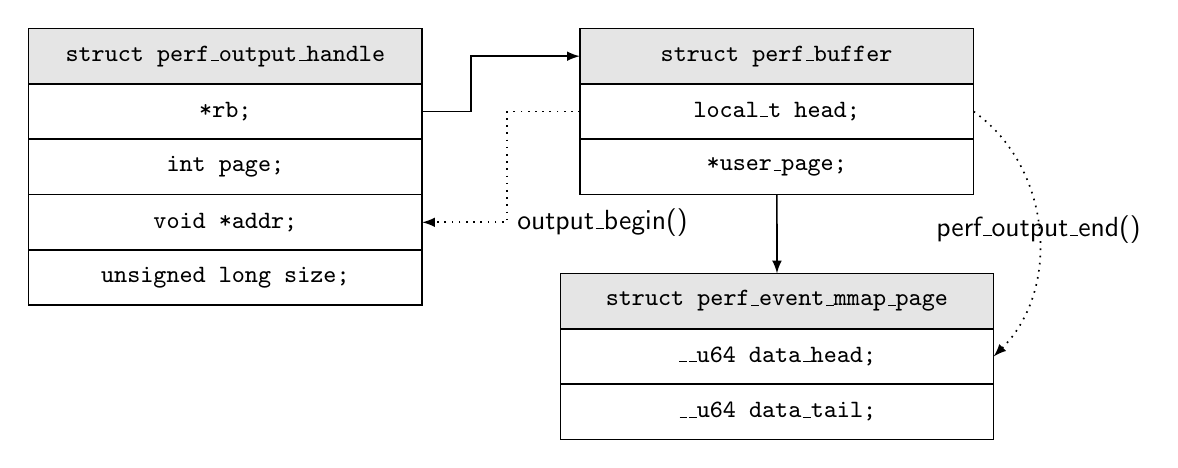
\begin{tikzpicture}[>=latex,font=\sffamily,semithick,scale=1.75]
	\node [minimum width=5cm,minimum height=2em,outer sep=0pt,draw=black,fill=gray!20] at (0,0) (oh) {\code{\small struct perf\_output\_handle}};
	\node [minimum width=5cm,minimum height=2em,outer sep=0pt,draw=black,fill=white,below=0cm of oh] (oh_rb) {\code{\small *rb;}};
	\node [minimum width=5cm,minimum height=2em,outer sep=0pt,draw=black,fill=white,below=0cm of oh_rb] (oh_page) {\code{\small int page;}};
	\node [minimum width=5cm,minimum height=2em,outer sep=0pt,draw=black,fill=white,below=0cm of oh_page] (oh_addr) {\code{\small void *addr;}};
	\node [minimum width=5cm,minimum height=2em,outer sep=0pt,draw=black,fill=white,below=0cm of oh_addr] (oh_size) {\code{\small unsigned long size;}};

	\node [minimum width=5cm,minimum height=2em,outer sep=0pt,draw=black,fill=gray!20,right=2cm of oh.east] (buf) {\code{\small struct perf\_buffer}};
	\node [minimum width=5cm,minimum height=2em,outer sep=0pt,draw=black,fill=white,below=0cm of buf] (buf_head) {\code{\small local\_t head;}};
	\node [minimum width=5cm,minimum height=2em,outer sep=0pt,draw=black,fill=white,below=0cm of buf_head] (buf_user_page) {\code{\small *user\_page;}};

	\node [minimum width=5.5cm,minimum height=2em,outer sep=0pt,draw=black,fill=gray!20,below=1cm of buf_user_page] (up) {\code{\small struct perf\_event\_mmap\_page}};
	\node [minimum width=5.5cm,minimum height=2em,outer sep=0pt,draw=black,fill=white,below=0cm of up] (up_head) {\code{\small \_\_u64 data\_head;}};
	\node [minimum width=5.5cm,minimum height=2em,outer sep=0pt,draw=black,fill=white,below=0cm of up_head] (up_tail) {\code{\small \_\_u64 data\_tail;}};

	\draw [->,semithick] (oh_rb.east) -- +(1em,0em) |- (buf.west);
	\draw [->,semithick] (buf_user_page.south) -- (up.north);
	\draw[->,dotted] (buf_head.east) to[bend left=50] node[midway] {perf\_output\_end()} (up_head.east);
	\draw[->,dotted] (buf_head.west) -- +(-1.5em,0em) |- node[midway,right] {output\_begin()} (oh_addr.east);
\end{tikzpicture}
\par
\textbf{Figure 7: Structures for writing ring buffer}
\end{center}

The event core layer in kernel uses the structure \code{perf\_buffer} to track the buffer's latest header, and it keeps the information for buffer pages.  If considering the life cycle, the structure \code{perf\_buffer} is allocated once the ring buffer is created, and it's released when the ring buffer is destroyed.

It's possible that multiple events to write buffer concurrently.  For instance, one software event and one hardware PMU event both are enabled for profiling, when the software event is in the middle of sampling, the hardware event maybe overflow and its interrupt is triggered in this case.  This leads to the race condition for \code{perf\_buffer::head}, because the software event sampling can be interrupted by the hardware event sampling.

Linux kernel uses compare-and-swap atomicity \code{local\_cmpxchg()} to implement the locklesss mechanism for protecting \code{perf\_buffer::head} (copied from \code{\_\_perf\_output\_begin()}):

\begin{lstlisting}
do {
        tail = READ_ONCE(rb->user_page->data_tail);
        offset = head = local_read(&rb->head);
        if (!rb->overwrite) {
                if (unlikely(!ring_buffer_has_space(head, tail,
                                                    perf_data_size(rb),
                                                    size, backward)))
                        goto fail;
        }

        /*
         * The above forms a control dependency barrier separating the
         * @tail load above from the data stores below. Since the @tail
         * load is required to compute the branch to fail below.
         *
         * A, matches D; the full memory barrier userspace SHOULD issue
         * after reading the data and before storing the new tail
         * position.
         *
         * See perf_output_put_handle().
         */

        if (!backward)
                head += size;
        else
                head -= size;
} while (local_cmpxchg(&rb->head, offset, head) != offset);
\end{lstlisting}

Comparing to \code{perf\_buffer}, the structure \code{perf\_output\_handle} is only used during the event sampling.  When an event is overflow, it firstly uses the structure \code{perf\_output\_handle} to establish a context for buffer's accessing, afterwards, sampling only uses the field \code{perf\_output\_handle::addr} as the destination address for copying sample data. 

A significant benefit from the structure \code{perf\_output\_handle} is it allows different events to write buffer concurrently.  Following the previous example, two copies of \code{perf\_output\_handle} work as two contexts for the software event and hardware event separately, thus every event reserves its own memory space in the function \code{out\_begin()} and \code{perf\_output\_handle::addr} is used for filling samples.

Until the sample data has been stored into buffer, the ring buffer's header is synced from \code{perf\_buffer::head} to \code{perf\_event\_mmap\_page::data\_head} in the function \code{perf\_output\_end()}.  This delivers the message to the perf tool that "now you are safe to read out the new samples from the user space".

\subsubsection*{Reading samples from buffer}

Like kernel's \code{perf\_output\_handle}, the structure \code{perf\_mmap} maintains a context for ring buffer in the user space, the context contains the info for buffer's start address, end address and mask; these values can be used to calculate the buffer pointer and size to be read based on different buffer modes.

The pointers and buffer are different data objects, it's possible for out-of-order accessing to them on the modern CPUs with relaxed memory model.  Furthermore, given perf and the profiled program running in multi-threads on multiple CPUs, the sequence between accessing pointers and buffer data must be promised by memory synchronization.

Besides the kernel function \code{perf\_output\_put\_handle()}, two helpers\\\code{ring\_buffer\_read\_head()} and \code{ring\_buffer\_write\_tail()} are introduced with memory barriers in the user space, they cooperates to ensure the data dependency; the rationale for the memory synchronization is:

\begin{tabular}{|l|l|}
\begin{minipage}{.4\textwidth}
\begin{lstlisting}[
tabsize=2,
numbersep=8pt,
numbers=left,
xleftmargin=0.5cm,frame=tlbr,framesep=2pt,framerule=0pt,
morekeywords ={class,run}
]
Kernel

if (LOAD ->data_tail) {
                   (A)
   STORE $data
   smp_wmb()       (B)
   STORE ->data_head
}
\end{lstlisting}
\end{minipage}

&

\begin{minipage}{.4\textwidth}
\begin{lstlisting}[
tabsize=2,
numbersep=8pt,
numbers=left,
xleftmargin=0.5cm,frame=tlbr,framesep=2pt,framerule=0pt,
aboveskip=-1.4\medskipamount,
morekeywords ={class,run}
]
User space

LOAD ->data_head
smp_rmb()       (C)
LOAD $data
smp_mb()        (D)
STORE ->data_tail
\end{lstlisting}
\end{minipage}
\end{tabular}

The comment in source file \code{include/linux/ring\_buffer.h} gives very nice description, here just tried to give explaination in my own words.

\code{(A)} indicates a control dependency between checking pointer \code{data\_tail} and filling sample, so that the kernel has chance to decide if the buffer has enough free space or not.  \code{(D)} needs to separate the ring buffer data reading from writing the pointer \code{data\_tail}, perf tool firstly reads samples and then tells kernel that samples have been consumed and it can safely use it from then on.  Since one of these two operations is reading and another is writing, thus it needs a full memory barrier.  \code{(B)} is a writing barrier in the middle of two writing operations, which makes sure the head pointer updating must be later than finishing current sampling.  \code{(C)} is a read memory barrier to split two read operations, it promises the program sequence for fetching the latest head pointer prior to reading samples.

\begin{lstlisting}
static inline u64 ring_buffer_read_head(struct perf_event_mmap_page *base)
{
/*
 * Architectures where smp_load_acquire() does not fallback to
 * READ_ONCE() + smp_mb() pair.
 */
#if defined(__x86_64__) || defined(__aarch64__) || defined(__powerpc64__) || \
    defined(__ia64__) || defined(__sparc__) && defined(__arch64__)
        return smp_load_acquire(&base->data_head);
#else
        u64 head = READ_ONCE(base->data_head);

        smp_rmb();
        return head;
#endif
}

static inline void ring_buffer_write_tail(struct perf_event_mmap_page *base,
                                          u64 tail)
{
        smp_store_release(&base->data_tail, tail);
}
\end{lstlisting}

Some architectures support one-way permeable barrier with load-acquire and store-release operations, these barriers are more relax to impose the barrier on any irrelevant memory operations, so \code{(C)} and \code{(D)} can be optimized to use barriers \code{smp\_load\_acquire()} and \code{smp\_store\_release()} respectively.

If an architecture doesn't support load-acquire and store-release, it will rollback to the old fashion with common memory barriers.  A minor improvement should be mentioned, as shown in \code{ring\_buffer\_read\_head()}, if an architecture doesn't support load-acquire primitive, it doesn't simply fallback to \code{READ\_ONCE() + smp\_mb()} encapsulated in \code{smp\_load\_acquire()}, the reason is it wants to benefit the performance by using a more lightweight barrier \code{smp\_rmb()} rather than \code{smp\_mb()}.

\section*{The mechanism for AUX ring buffer}

This chapter will examine the implementation for AUX ring buffer.  It firstly concludes the relationship between the AUX ring buffer and the generic ring buffer;  then it reviews how the AUX ring buffer co-work with the generic ring buffer, and what's the extension introduced by the AUX ring buffer for the sampling mechanism.

\subsection*{The relationship with the generic ring buffer}

In an overview, the AUX ring buffer is an auxiliary for the generic ring buffer.  The generic ring buffer is primarily used to store the event samples, and every event fromat complies with the definition in the union \code{perf\_event}; the AUX ring buffer is for recording the hardware tracing, and the trace data format is hardware IP dependent.  The advantage of introducing AUX ring buffer is it can de-couple the data transferring between the generic perf events and the hardware tracing.

It's nature for the AUX ring buffer to reuse the same algorithm with the generic ring buffer for the buffer management.  The control stucture \code{perf\_event\_mmap\_page} extends the new fields \code{aux\_head} and \code{aux\_tail} for the head and tail pointers of the AUX ring buffer.

The record option \code{record\_opts::auxtrace\_mmap\_pages} is set during the AUX trace initialisation, otherwise, if perf session has not attached to any AUX trace, this option is the default value '0'.  When it is a non-zero value, the function \code{auxtrace\_mmap\_\_mmap()} invokes system call mmap() and the kernel function \code{rb\_alloc\_aux()} serves for allocating pages; these pages will be deferred to map into VMA when detects the page fault which is the exactly same mechanism with the generic ring buffer.  As the result, the perf tool have two types of ring buffer and needs to manage every ring buffer individually.

\begin{center}
\par
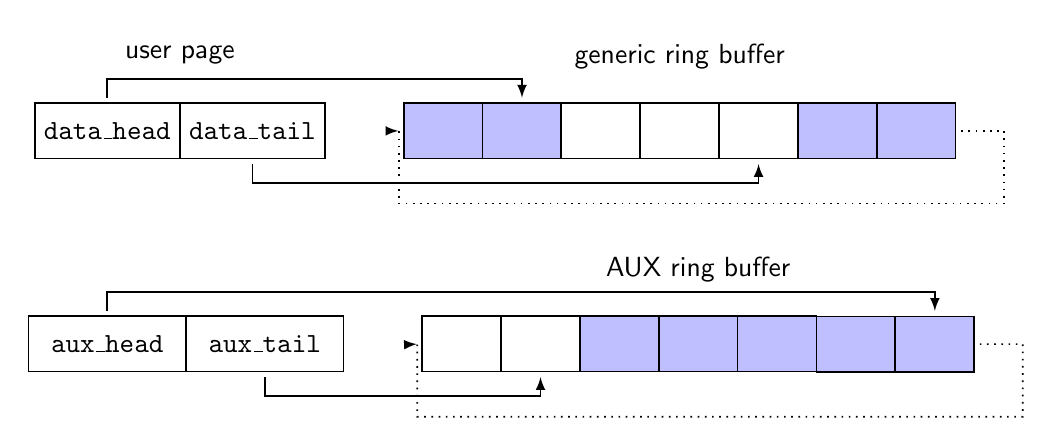
\begin{tikzpicture}[>=latex,font=\sffamily,semithick,scale=1.75]
	\node [minimum width=1cm,minimum height=2em,outer sep=0pt,draw=black,fill=white] at (0,0) (A) {\code{data\_head}};
	\node [minimum height=2em] at (A.east) (A2) {};
	\node [minimum width=1cm,minimum height=2em,outer sep=0pt,draw=black,fill=white,anchor=west] at (A.east) (B) {\code{data\_tail}};
        \node [minimum width=1cm,minimum height=2em,outer sep=0pt,draw=black,fill=blue!25,right=1cm of B] (C) {};
        \node [minimum width=1cm,minimum height=2em,outer sep=0pt,draw=black,fill=blue!25,anchor=west] at (C.east) (D) {};
        \node [minimum width=1cm,minimum height=2em,outer sep=0pt,draw=black,fill=white,anchor=west] at (D.east) (E) {};
        \node [minimum width=1cm,minimum height=2em,outer sep=0pt,draw=black,fill=white,anchor=west] at (E.east) (F) {};
        \node [minimum width=1cm,minimum height=2em,outer sep=0pt,draw=black,fill=white,anchor=west] at (F.east) (G) {};
        \node [minimum width=1cm,minimum height=2em,outer sep=0pt,draw=black,fill=blue!25,anchor=west] at (G.east) (H) {};
        \node [minimum width=1cm,minimum height=2em,outer sep=0pt,draw=black,fill=blue!25,anchor=west] at (H.east) (I) {};
	\node [minimum width=1cm,minimum height=2em,outer sep=0pt,above=0.7em of A2] (control) {user page};
	\node [minimum width=1cm,minimum height=2em,outer sep=0pt,above=0.7em of F] (buffer) {generic ring buffer};
	\draw [->,shorten >=2pt,shorten <=2pt,semithick,dotted] (I.east) -- +(1em,0em) -- +(1em,-1.5em) -- +(-11.5em,-1.5em) -- +(-11.5em,0em) -- (C.west);
	\draw [->,shorten >=2pt,shorten <=2pt,semithick] (A.north) -- +(0em,.5em) -| (D.north);
	\draw [->,shorten >=2pt,shorten <=2pt,semithick] (B.south) -- +(0em,-.5em) -| (G.south);

	\node [minimum width=2cm,minimum height=2em,outer sep=0pt,draw=black,fill=white,below=2cm of A] (AA) {\code{aux\_head}};
	\node [minimum width=2cm,minimum height=2em,outer sep=0pt,draw=black,fill=white,anchor=west] at (AA.east) (BB) {\code{aux\_tail}};
        \node [minimum width=1cm,minimum height=2em,outer sep=0pt,draw=black,fill=white,right=1cm of BB] (CC) {};
        \node [minimum width=1cm,minimum height=2em,outer sep=0pt,draw=black,fill=white,anchor=west] at (CC.east) (DD) {};
        \node [minimum width=1cm,minimum height=2em,outer sep=0pt,draw=black,fill=blue!25,anchor=west] at (DD.east) (EE) {};
        \node [minimum width=1cm,minimum height=2em,outer sep=0pt,draw=black,fill=blue!25,anchor=west] at (EE.east) (FF) {};
        \node [minimum width=1cm,minimum height=2em,outer sep=0pt,draw=black,fill=blue!25,anchor=west] at (FF.east) (GG) {};
        \node [minimum width=1cm,minimum height=2em,outer sep=0pt,draw=black,fill=blue!25,anchor=west] at (GG.east) (HH) {};
        \node [minimum width=1cm,minimum height=2em,outer sep=0pt,draw=black,fill=blue!25,anchor=west] at (HH.east) (II) {};
	\node [minimum width=1cm,minimum height=2em,outer sep=0pt,above=0.7em of FF] (buffer2) {AUX ring buffer};
	\draw [->,shorten >=2pt,shorten <=2pt,semithick,dotted] (II.east) -- +(1em,0em) -- +(1em,-1.5em) -- +(-11.5em,-1.5em) -- +(-11.5em,0em) -- (CC.west);
	\draw [->,shorten >=2pt,shorten <=2pt,semithick] (AA.north) -- +(0em,.5em) -| (II.north);
	\draw [->,shorten >=2pt,shorten <=2pt,semithick] (BB.south) -- +(0em,-.5em) -| (DD.south);

\end{tikzpicture}
\par
\textbf{Figure 8: Perf generic ring buffer and AUX ring buffer}
\end{center}

An interesting question is: Is it possible to only allocate the AUX ring buffer for hardware trace if there have no any other PMU events opened?  Say below command only enables Arm CoreSight event:

\code{\\\indent perf record -e cs\_etm/@tmc\_etr0/u --a program\\}


In fact, the generic ring buffer and AUX ring buffer are allocated in pairs, even when only the hardware trace event is enabled (see \code{mmap\_\_mmap()}).  The reason is the generic ring buffer is not merely for event sampling, it also records the process memory mapping so that the info can be used for parsing symbols, and the AUX event will be saved into the generic ring buffer as well.  The AUX event and AUX trace data will be addressed in details in the later section.

Now let's review the AUX ring buffer deployment for perf modes.  I.e., for per thread mode, perf tool only allocates one generic ring buffer and one AUX ring buffer for the whole session; for the system wide mode, perf allocates the generic ring buffer and the AUX ring buffer per CPU wise.  The figure demonstrates the buffers layout in the system wide mode; if there have any activities on one CPU, the event samples and the hardware trace data are recorded into the dedicated buffers for the CPU.

\begin{center}
\par
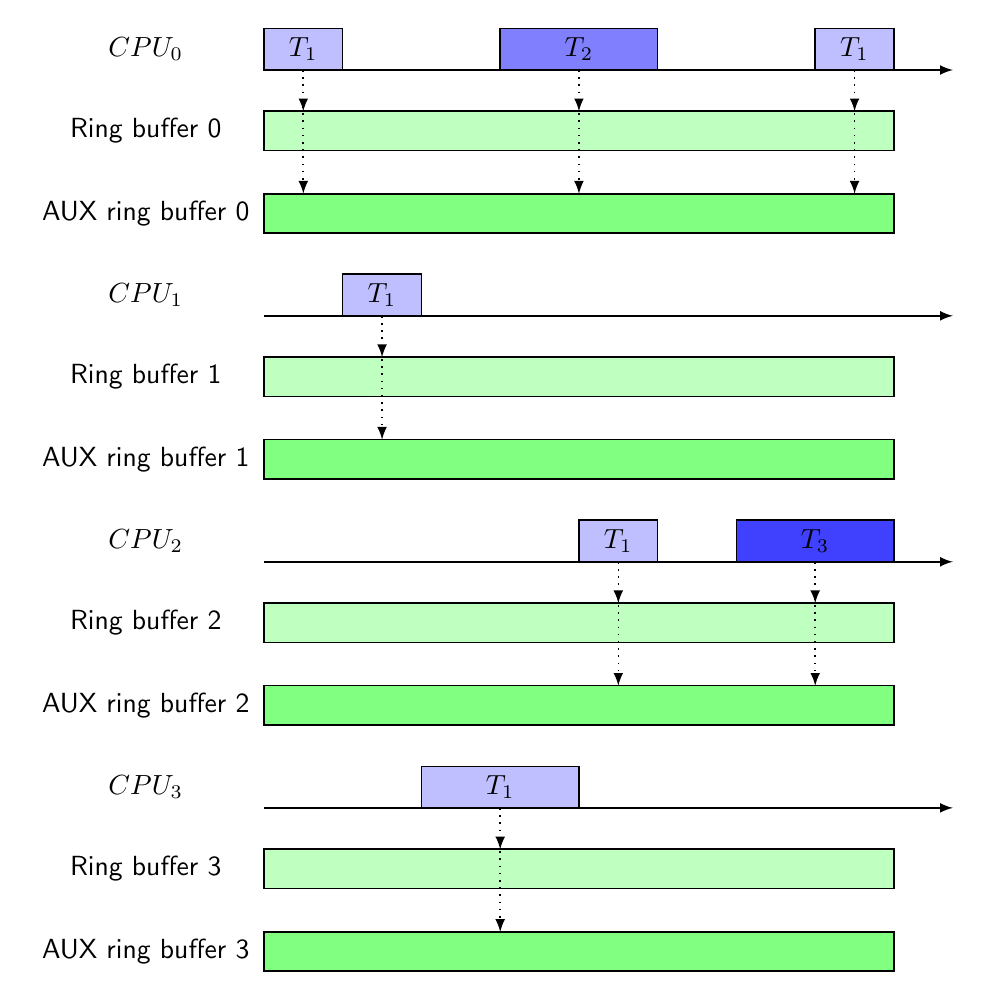
\begin{tikzpicture}[>=latex,font=\sffamily,semithick,scale=1.75]
	\node [minimum width=3cm,minimum height=.5cm,outer sep=0pt] at (0,0) (cpu0) {\( CPU_0 \)};
	\node [minimum width=1cm,minimum height=.5cm,outer sep=0pt,draw=black,fill=blue!25,right=0cm of cpu0] at (cpu0.east) (cpu0_p1_0) {\(T_{1}\)};
	\node [minimum width=2cm,minimum height=.5cm,outer sep=0pt,draw=black,fill=blue!50,right=3cm of cpu0] at (cpu0.east) (cpu0_p2_0) {\(T_{2}\)};
	\node [minimum width=1cm,minimum height=.5cm,outer sep=0pt,draw=black,fill=blue!25,right=7cm of cpu0] (cpu0_p1_1) {\(T_{1}\)};
	\draw[->] (cpu0.south east) -- +(5cm,0);

	\node [minimum width=3cm,minimum height=.5cm,outer sep=0pt,below=.5cm of cpu0] (rb0_txt) {Ring buffer 0};
	\node [minimum width=8cm,minimum height=.5cm,outer sep=0pt,draw=black,fill=green!25,right=0cm of rb0_txt] (rb0) {};

	\node [minimum width=3cm,minimum height=.5cm,outer sep=0pt,below=.5cm of rb0_txt] (aux_rb0_txt) {AUX ring buffer 0};
	\node [minimum width=8cm,minimum height=.5cm,outer sep=0pt,draw=black,fill=green!50,right=0cm of aux_rb0_txt] (aux_rb0) {};

	\node [minimum width=3cm,minimum height=.5cm,outer sep=0pt,below=.5cm of aux_rb0_txt] (cpu1) {\(CPU_{1}\)};
	\node [minimum width=1cm,minimum height=.5cm,outer sep=0pt,draw=black,fill=blue!25,right=1cm of cpu1] at (cpu1.east) (cpu1_p1_0) {\(T_{1}\)};
	\draw[->] (cpu1.south east) -- +(5cm,0);

	\node [minimum width=3cm,minimum height=.5cm,outer sep=0pt,below=.5cm of cpu1] (rb1_txt) {Ring buffer 1};
	\node [minimum width=8cm,minimum height=.5cm,outer sep=0pt,draw=black,fill=green!25,right=0cm of rb1_txt] (rb1) {};

	\node [minimum width=3cm,minimum height=.5cm,outer sep=0pt,below=.5cm of rb1_txt] (aux_rb1_txt) {AUX ring buffer 1};
	\node [minimum width=8cm,minimum height=.5cm,outer sep=0pt,draw=black,fill=green!50,right=0cm of aux_rb1_txt] (aux_rb1) {};

	\node [minimum width=3cm,minimum height=.5cm,outer sep=0pt,below=.5cm of aux_rb1_txt] (cpu2) {\(CPU_{2}\)};
	\node [minimum width=1cm,minimum height=.5cm,outer sep=0pt,draw=black,fill=blue!25,right=4cm of cpu2] (cpu2_p1_0) {\(T_{1}\)};
	\node [minimum width=2cm,minimum height=.5cm,outer sep=0pt,draw=black,fill=blue!75,right=6cm of cpu2] (cpu2_p3_0) {\(T_{3}\)};
	\draw[->] (cpu2.south east) -- +(5cm,0);

	\node [minimum width=3cm,minimum height=.5cm,outer sep=0pt,below=.5cm of cpu2] (rb2_txt) {Ring buffer 2};
	\node [minimum width=8cm,minimum height=.5cm,outer sep=0pt,draw=black,fill=green!25,right=0cm of rb2_txt] (rb2) {};

	\node [minimum width=3cm,minimum height=.5cm,outer sep=0pt,below=.5cm of rb2_txt] (aux_rb2_txt) {AUX ring buffer 2};
	\node [minimum width=8cm,minimum height=.5cm,outer sep=0pt,draw=black,fill=green!50,right=0cm of aux_rb2_txt] (aux_rb2) {};

	\node [minimum width=3cm,minimum height=.5cm,outer sep=0pt,below=.5cm of aux_rb2_txt] (cpu3) {\(CPU_{3}\)};
	\node [minimum width=2cm,minimum height=.5cm,outer sep=0pt,draw=black,fill=blue!25,right=2cm of cpu3] (cpu3_p1_0) {\(T_{1}\)};
	\draw[->] (cpu3.south east) -- +(5cm,0);

	\node [minimum width=3cm,minimum height=.5cm,outer sep=0pt,below=.5cm of cpu3] (rb3_txt) {Ring buffer 3};
	\node [minimum width=8cm,minimum height=.5cm,outer sep=0pt,draw=black,fill=green!25,right=0cm of rb3_txt] (rb3) {};

	\node [minimum width=3cm,minimum height=.5cm,outer sep=0pt,below=.5cm of rb3_txt] (aux_rb3_txt) {AUX ring buffer 3};
	\node [minimum width=8cm,minimum height=.5cm,outer sep=0pt,draw=black,fill=green!50,right=0cm of aux_rb3_txt] (aux_rb3) {};

	\draw[->,dotted] (cpu0_p1_0.south) -- (cpu0_p1_0.south|-rb0.north);
	\draw[->,dotted] (cpu0_p1_1.south) -- (cpu0_p1_1.south|-rb0.north);
	\draw[->,dotted] (cpu0_p2_0.south) -- (cpu0_p2_0.south|-rb0.north);

	\draw[->,dotted] (cpu0_p1_0.south) -- (cpu0_p1_0.south|-aux_rb0.north);
	\draw[->,dotted] (cpu0_p1_1.south) -- (cpu0_p1_1.south|-aux_rb0.north);
	\draw[->,dotted] (cpu0_p2_0.south) -- (cpu0_p2_0.south|-aux_rb0.north);

	\draw[->,dotted] (cpu1_p1_0.south) -- (cpu1_p1_0.south|-rb1.north);

	\draw[->,dotted] (cpu1_p1_0.south) -- (cpu1_p1_0.south|-aux_rb1.north);

	\draw[->,dotted] (cpu2_p1_0.south) -- (cpu2_p1_0.south|-rb2.north);
	\draw[->,dotted] (cpu2_p3_0.south) -- (cpu2_p3_0.south|-rb2.north);

	\draw[->,dotted] (cpu2_p1_0.south) -- (cpu2_p1_0.south|-aux_rb2.north);
	\draw[->,dotted] (cpu2_p3_0.south) -- (cpu2_p3_0.south|-aux_rb2.north);

	\draw[->,dotted] (cpu3_p1_0.south) -- (cpu3_p1_0.south|-rb3.north);

	\draw[->,dotted] (cpu3_p1_0.south) -- (cpu3_p1_0.south|-aux_rb3.north);
\end{tikzpicture}
\par
\textbf{Figure 9: Ring buffers for system wide mode}
\end{center}

\subsection*{AUX events}

Similiar to \code{perf\_output\_begin()} and \code{perf\_output\_end()} for the generic ring buffer, the functions \code{perf\_aux\_output\_begin()} and \code{perf\_aux\_output\_end()} works as AUX ring buffer variant for processing the hardware trace data.

Same as the generic ring bufer, the structure \code{perf\_output\_handle} is used as a context to track the AUX buffer's info.  Unlike \code{perf\_output\_begin()} allocates the buffer for only one sample, \code{perf\_aux\_output\_begin()} creates the context and allocate all available buffer for filling AUX trace data.

The function \code{perf\_aux\_output\_end()} finishes two things:
\begin{itemize}
	\item It fills an event \code{PERF\_RECORD\_AUX} into the generic ring buffer, this event delivers the information of the start address and data size for a chunk of hardware trace data has been stored into the AUX ring buffer;
	\item The driver has stored new trace data into the AUX ring buffer, the argument \code{size} indicates how many bytes have been consumed by the hardware tracing, thus \code{perf\_aux\_output\_end()} updates the header pointer to reflect the latest buffer usage.
\end{itemize}

There have two occasions to wake up the perf tool for reading out AUX trace data.  Except the event \code{PERF\_RECORD\_AUX} can wake up the perf process, if the AUX trace size beyonds the watermark, the kernel also wakes up the perf process to fetch AUX trace data.

Perf tool saves events continuously in data file, the event \code{PERF\_RECORD\_AUX} is saved same as any other events.  But the event \code{PERF\_RECORD\_AUX} doesn't contain any AUX trace data, it just presents a single recording event occurring in the kernel, and if the AUX ring buffer is big enough, it's possible that the multiple \code{PERF\_RECORD\_AUX} events occured prior to wake up the perf tool to handle the AUX ring buffer.

\begin{center}
\par
\begin{tikzpicture}[>=latex,font=\sffamily,semithick,scale=1.75]
	\node [minimum width=3cm,minimum height=.5cm,outer sep=0pt,below=.5cm of cpu0] at (0,0) (rb0_txt) {Ring buffer 0};
	\node [minimum width=1cm,minimum height=.5cm,outer sep=0pt,draw=black,fill=green!25,right=.5cm of rb0_txt] at (rb0_txt.east) (rb0_1) {...};
	\node [minimum width=3cm,minimum height=.5cm,outer sep=0pt,draw=black,fill=green!25,anchor=west] at (rb0_1.east) (rb0_2) {\tiny \(PERF\_RECORD\_AUX\)};
	\node [minimum width=1cm,minimum height=.5cm,outer sep=0pt,draw=black,fill=green!25,anchor=west] at (rb0_2.east) (rb0_3) {...};
	\node [minimum width=3cm,minimum height=.5cm,outer sep=0pt,draw=black,fill=green!25,anchor=west] at (rb0_3.east) (rb0_4) {\tiny \(PERF\_RECORD\_AUX\)};
	\node [minimum width=1cm,minimum height=.5cm,outer sep=0pt,draw=black,fill=green!25,anchor=west] at (rb0_4.east) (rb0_5) {...};

	\node [minimum width=3cm,minimum height=.5cm,outer sep=0pt,below=.5cm of rb0_txt] (aux_rb0_txt) {AUX ring buffer 0};
	\node [minimum width=2cm,minimum height=.5cm,outer sep=0pt,draw=black,fill=green!50,anchor=west,right=2.5cm of aux_rb0_txt] (aux_rb0_1) {};
	\node [minimum width=4cm,minimum height=.5cm,outer sep=0pt,draw=black,fill=green!50,anchor=west] at (aux_rb0_1.east) (aux_rb0_2) {};

	\node [minimum width=3cm,minimum height=.5cm,outer sep=0pt,below=1cm of aux_rb0_txt] (data) {Perf data file};
	\node [minimum width=.5cm,minimum height=.5cm,outer sep=0pt,draw=black,,right=3cm of data] at (data.east) (data_1) {...};
	\node [minimum width=.5cm,minimum height=.5cm,outer sep=0pt,draw=black,anchor=west] at (data_1.east) (data_2) {...};
	\node [minimum width=.5cm,minimum height=.5cm,outer sep=0pt,draw=black,anchor=west] at (data_2.east) (data_3) {...};
	\node [minimum width=.5cm,minimum height=.5cm,outer sep=0pt,draw=black,anchor=west] at (data_3.east) (data_4) {...};
	\node [minimum width=.5cm,minimum height=.5cm,outer sep=0pt,draw=black,anchor=west] at (data_4.east) (data_5) {...};
	\node [minimum width=.5cm,minimum height=.5cm,outer sep=0pt,draw=black,anchor=west] at (data_5.east) (data_6) {...};

	\draw [->,semithick] (rb0_1.west) -- +(-.5em,0em) |- (data_1.west);
	\draw [->,dotted] (rb0_2.south) -- +(0em,-.3em) -| (aux_rb0_1.north);
	\draw [->,dotted] (rb0_4.south) -- +(0em,-.3em) -| (aux_rb0_2.north);

	\draw [->,semithick] (aux_rb0_1.south) -- +(0em,-.8em) -| (data_4.north);
	\draw [->,semithick] (aux_rb0_2.south) -- +(0em,-.8em) node[right,align=left,yshift=0cm,font=\tiny] {PERF\_RECORD\_AUXTRACE\\is synthesized in perf when\\record AUX trace data} -| (data_4.north);

\end{tikzpicture}
\par
\textbf{Figure 10: AUX events \code{PERF\_RECORD\_AUX} and \code{PERF\_RECORD\_AUXTRACE}}
\end{center}

Perf needs to give out a clear boundary that "hey, this chunk in the perf file is the AUX trace data" when saves the AUX trace data into perf file and afterwards can be easily parsed in the post analysis.  For this reason, perf tool synthesizes an event \code{PERF\_RECORD\_AUXTRACE} which combines the event header and AUX trace data.

\subsection*{Snapshot mode}

Perf provides snapshot mode for AUX ring buffer, in this mode, users can only record AUX trace data at a specific time point which users are interested in.  E.g. if an user wants to record the AUX trace data periodically with 1 second interval, it can use commands:

\begin{lstlisting}
	perf record -e cs_etm/@tmc_etr0/u -S -a program &
	PERFPID=$!
	while true; do
		kill -USR2 $PERFPID
		sleep 1
	done
\end{lstlisting}

Let's firstly answer serveral questions to make clear the concept for snapshot: what's the snapshot and what's relationship between the snapsthot mode and the existed perf modes?  The snapshot mode is only relevant to how to record the AUX tracing data, it is no matter with the ring buffers deployment.  As we know, the buffers deployment is decided by per thread mode, per CPU mode or system wide mode, and the snapshot can be applied to any of these modes.

\begin{center}
\par
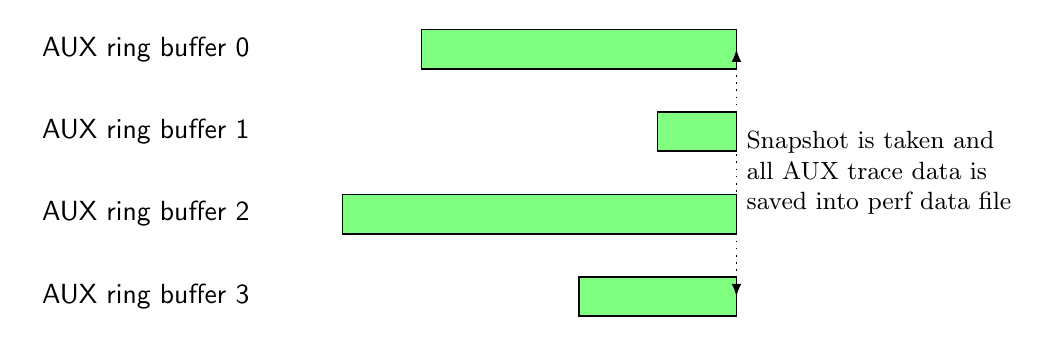
\begin{tikzpicture}[>=latex,font=\sffamily,semithick,scale=1.75]
	\node [minimum width=3cm,minimum height=.5cm,outer sep=0pt] at (0,0) (aux_rb0_txt) {AUX ring buffer 0};
	\node [minimum width=4cm,minimum height=.5cm,outer sep=0pt,draw=black,fill=green!50,right=2cm of aux_rb0_txt] (aux_rb0) {};

	\node [minimum width=3cm,minimum height=.5cm,outer sep=0pt,below=.5cm of aux_rb0_txt] (aux_rb1_txt) {AUX ring buffer 1};
	\node [minimum width=1cm,minimum height=.5cm,outer sep=0pt,draw=black,fill=green!50,right=5cm of aux_rb1_txt] (aux_rb1) {};

	\node [minimum width=3cm,minimum height=.5cm,outer sep=0pt,below=.5cm of aux_rb1_txt] (aux_rb2_txt) {AUX ring buffer 2};
	\node [minimum width=5cm,minimum height=.5cm,outer sep=0pt,draw=black,fill=green!50,right=1cm of aux_rb2_txt] (aux_rb2) {};

	\node [minimum width=3cm,minimum height=.5cm,outer sep=0pt,below=.5cm of aux_rb2_txt] (aux_rb3_txt) {AUX ring buffer 3};
	\node [minimum width=2cm,minimum height=.5cm,outer sep=0pt,draw=black,fill=green!50,right=4cm of aux_rb3_txt] (aux_rb3) {};

	\draw[<->,dotted] (aux_rb0.east) -- node[right,align=left,yshift=0cm,font=\small] {Snapshot is taken and \\all AUX trace data is\\ saved into perf data file} (aux_rb3.east);
\end{tikzpicture}
\par
\textbf{Figure 11: Snapshot with system wide mode}
\end{center}

The main flow for snapshot is:

\begin{itemize}
	\item Before the snapshot is taken, the AUX ring buffer runs in free mode; there have no the AUX event and the trace date will not be saved into the perf data file;
	\item When the user takes a snapshot for the profiling, it sends \code{USR2} signal to perf, perf will invoke the callback \code{auxtrace\_record::snapshot\_start()} to disable the hardware tracing; in the kernel the driver fills the hardware trace data into the AUX ring buffer and the event \code{PERF\_RECORD\_AUX} is saved in the generic ring buffer;
	\item \code{record\_\_read\_auxtrace\_snapshot()} reads out the hardware trace data from AUX ring buffer, and saves into perf data file; during this process, the callback \code{auxtrace\_record::find\_snapshot()} is used to calculate the head and old head, these two heads will be described soon;
	\item After the snapshot is finished, \code{auxtrace\_record::snapshot\_finish()} will restart the PMU event for AUX tracing, so the hardware will generate new trace data.
\end{itemize}

A prominent difference for snapshot is it only uses the head pointer \code{aux\_head} and doesn't update tail pointer \code{aux\_tail}.  The AUX ring buffer is possible that has not been overflow when snapshot, but if users take enough time for running the profiled program before taking snapshot, the AUX ring buffer can be filled with the AUX trace data for one or even multiple rounds, therefore the tail pointer is useless and perf doesn't maintain it for snapshot mode.  The AUX trace data size calculation is specific for AUX event, so the callback \code{auxtrace\_record::find\_snapshot()} is introduced, it needs to judge the head pointer has been wrapped around or not, and fixes up the head and the "old" head based on different situations.

\section*{Arm CoreSight: an example for using AUX ring buffer}

This chapter reviews how Arm CoreSight uses AUX ring buffer (as writing this document the kernel's latest version is v5.13, all the discussion is based on the code in this version).  It uses bottom-up approach to go through the Arm CoreSight implementation: it firstly summarizes the underlying hardware design, and then describes the implementation for how Arm CoreSight integrates the AUX ring buffer in details.

\subsection*{Recap for Arm CoreSight}

The Arm architecture refers to a processor or core as a Processing Element (PE), any PE connected to a tracer can be recroded for its program flow by the tracer; the tracer is named as Embedded Trace Macrocell (ETM), nowdays the commonly used tracer IP is ETMv4 for Armv8 CPUs.

The data path is required for outputting trace data, a data path is established by links between tracers and sinks, a link can be a funnel or a replicator; a funnel is used to pass multiple tracers to a sink, and a replicator can be used to distribute the same source to different sinks.

The end point is a sink, different sinks are for different target medias.  A sink can be Trace Port Interface Units (TPIUs) for dumping trace data to high speed port so the trace data can be captured by external debugger tool, Embedded Trace Buffers (ETB) for saving trace data to SRAM or Trace Memory Controllers (TMC) for accessing SDRAM.

Of course, the up description is highly condensed and it just wants to create a simplized hardware model to give readers a sense for how the CoreSight works with different components; the realistic hardware is much more complex.

Let's focus on the AUX ring buffer implementation, so we will take close look at TMC which uses the system memory for outputting trace data.

\subsection*{Three memory modes for Trace Memory Controllers (TMC)}

TMC supports three memory modes: flat mode, scatter-gather mode, and Coresight Address Translation Unit (CATU) mode.

The memory modes can be divided into two kinds of pages allocation.  The flat mode asks to allocate memory with physical continuous pages, TMC directly access the memory region based on the physical address.  For scatter-gather mode and CATU mode, both supports the scatter-list pages, this gives the flexibility for using the discontinuous pages and relies on translation table for accessing physical pages.

Comparing against the scatter-gather mode, the CATU mode is improved for the physical address space length.  The translation table entry is extended from scatter-gather mode's 32 bits to CATU mode's 64 bits, the scatter-gather mode only can support maximum to 40 bits of physical address space (the table entry's bit4-bit31 are mapped to physcial address bit12-bit39), in opposition CATU supports 64 bits of physical address space.

\begin{center}
\par
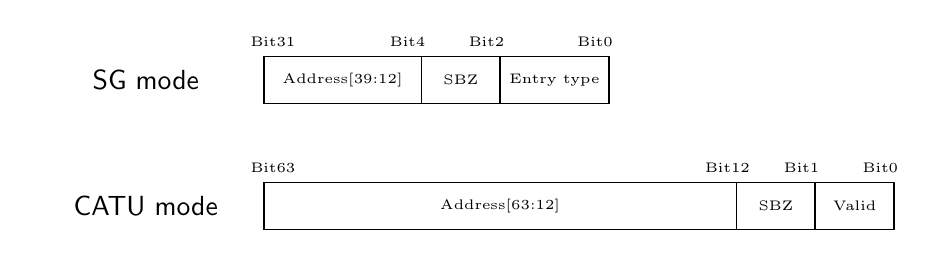
\begin{tikzpicture}[>=latex,font=\sffamily,semithick,scale=1.75]
	\node [minimum width=3cm,minimum height=.6cm,outer sep=0pt] at (0,0) (sg_mode) {SG mode};
	\node [minimum width=2cm,minimum height=.6cm,outer sep=0pt,draw=black,right=0cm of sg_mode,font=\tiny] (sg_address) {Address[39:12]};
	\node [minimum width=1cm,minimum height=.6cm,outer sep=0pt,draw=black,anchor=west,font=\tiny] at (sg_address.east) (sg_sbz) {SBZ};
	\node [minimum width=1cm,minimum height=.6cm,outer sep=0pt,draw=black,anchor=west,font=\tiny] at (sg_sbz.east) (sg_type) {Entry type};

	\node [minimum width=3cm,minimum height=.6cm,outer sep=0pt,below=1cm of sg_mode] (catu_mode) {CATU mode};
	\node [minimum width=6cm,minimum height=.6cm,outer sep=0pt,draw=black,right=0cm of catu_mode,font=\tiny] (catu_address) {Address[63:12]};
	\node [minimum width=1cm,minimum height=.6cm,outer sep=0pt,draw=black,anchor=west,font=\tiny] at (catu_address.east) (catu_sbz) {SBZ};
	\node [minimum width=1cm,minimum height=.6cm,outer sep=0pt,draw=black,anchor=west,font=\tiny] at (catu_sbz.east) (catu_valid) {Valid};

	\node [above right = 0em and -1.5em of sg_type,font=\tiny] (lable1) {Bit0};
	\node [above right = 0em and -1.5em of sg_sbz,font=\tiny] (lable1) {Bit2};
	\node [above right = 0em and -1.5em of sg_address,font=\tiny] (lable1) {Bit4};
	\node [above left = 0em and -1.5em of sg_address,font=\tiny] (lable1) {Bit31};

	\node [above right = 0em and -1.5em of catu_valid,font=\tiny] (lable1) {Bit0};
	\node [above right = 0em and -1.5em of catu_sbz,font=\tiny] (lable1) {Bit1};
	\node [above right = 0em and -1.5em of catu_address,font=\tiny] (lable1) {Bit12};
	\node [above left = 0em and -1.5em of catu_address,font=\tiny] (lable1) {Bit63};
\end{tikzpicture}
\par
\textbf{Figure 12: Table entry format for SG and CATU modes}
\end{center}

\subsection*{Implementation AUX ring buffer for Arm CoreSight}

Below four callbacks in the structure \code{pmu} play important roles for manipulating the AUX ring buffer.

\begin{lstlisting}
int __init etm_perf_init(void)
{
        [...]

        etm_pmu.setup_aux               = etm_setup_aux;
        etm_pmu.free_aux                = etm_free_aux;
        etm_pmu.start                   = etm_event_start;
        etm_pmu.stop                    = etm_event_stop;

        [...]
}
\end{lstlisting}

As mentioned the AUX ring buffer has been allocated by \code{rb\_alloc\_aux()}, the original design anticipates calling \code{pmu::setup\_aux()} to setup the PMU private data structures for the AUX ring buffer, e.g. creates the translation table for scatter-gather pages so that the sink can directly access the AUX ring buffer.

Unfortunately, Arm CoreSight's flat mode cannot support the scatter-gather pages, the solution is the function \code{etm\_setup\_aux()} invokes\\\code{sink\_ops(sink)->alloc\_buffer()}, the sink operation \code{sink\_ops(sink)} is dynamically assigned based on the memory mode, whatever which mode is in use, the low level callback \code{sink\_ops(sink)->alloc\_buffer()} allocates a bounce buffer, at the end TMC rountes trace data into the bounce buffer.

It's easy to understand for applying the bounce buffer for flat mode; it's questionable for SG and CATU modes, which have already support scatter-gather list from the hardware design but why still use the bounce buffer in the software code?  A reason is that this allows the implementation is general for all of these three modes, and the code is neat enough for later optimization.

\begin{center}
\par
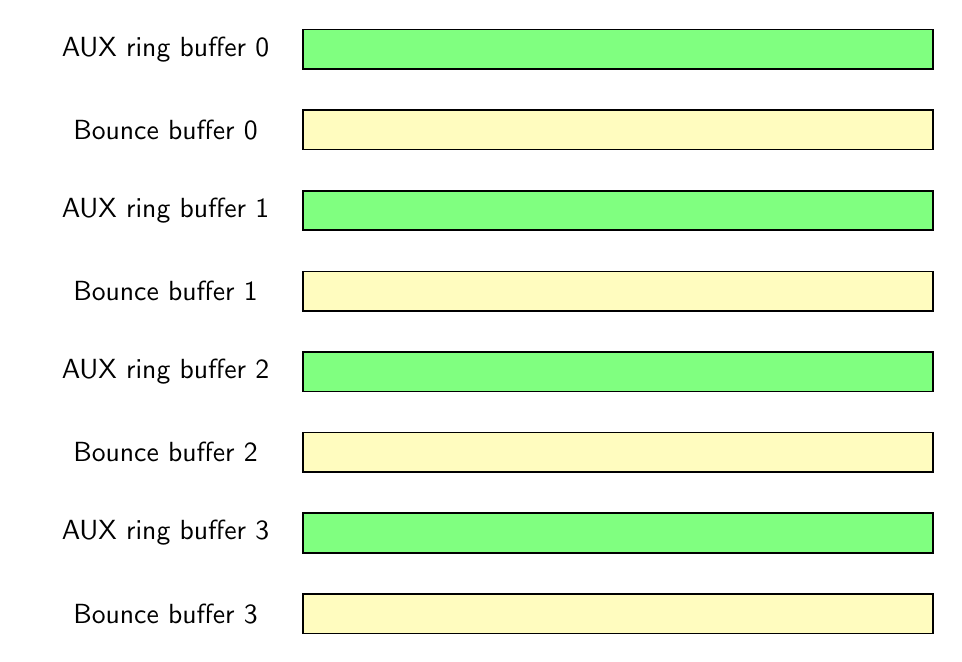
\begin{tikzpicture}[>=latex,font=\sffamily,semithick,scale=1.75]
	\node [minimum width=3.5cm,minimum height=.5cm,outer sep=0pt] at (0,0) (aux_rb0_txt) {AUX ring buffer 0};
	\node [minimum width=8cm,minimum height=.5cm,outer sep=0pt,draw=black,fill=green!50,right=0cm of aux_rb0_txt] (aux_rb0_0) {};

	\node [minimum width=3.5cm,minimum height=.5cm,outer sep=0pt,below=.5cm of aux_rb0_txt] (bounce_buf0_txt) {Bounce buffer 0};
	\node [minimum width=8cm,minimum height=.5cm,outer sep=0pt,draw=black,fill=yellow!25,right=0cm of bounce_buf0_txt] (boun_buf0_0) {};

	\node [minimum width=3.5cm,minimum height=.5cm,outer sep=0pt,below=.5cm of bounce_buf0_txt] (aux_rb1_txt) {AUX ring buffer 1};
	\node [minimum width=8cm,minimum height=.5cm,outer sep=0pt,draw=black,right=0cm of aux_rb1_txt,fill=green!50] (aux_rb1_0) {};

	\node [minimum width=3.5cm,minimum height=.5cm,outer sep=0pt,below=.5cm of aux_rb1_txt] (bounce_buf1_txt) {Bounce buffer 1};
	\node [minimum width=8cm,minimum height=.5cm,outer sep=0pt,draw=black,right=0cm of bounce_buf1_txt,fill=yellow!25] (boun_buf1_0) {};

	\node [minimum width=3.5cm,minimum height=.5cm,outer sep=0pt,below=.5cm of bounce_buf1_txt] (aux_rb2_txt) {AUX ring buffer 2};
	\node [minimum width=8cm,minimum height=.5cm,outer sep=0pt,draw=black,right=0cm of aux_rb2_txt,fill=green!50] (aux_rb2_0) {};

	\node [minimum width=3.5cm,minimum height=.5cm,outer sep=0pt,below=.5cm of aux_rb2_txt] (bounce_buf2_txt) {Bounce buffer 2};
	\node [minimum width=8cm,minimum height=.5cm,outer sep=0pt,draw=black,right=0cm of bounce_buf2_txt,fill=yellow!25] (boun_buf2_0) {};

	\node [minimum width=3.5cm,minimum height=.5cm,outer sep=0pt,below=.5cm of bounce_buf2_txt] (aux_rb3_txt) {AUX ring buffer 3};
	\node [minimum width=8cm,minimum height=.5cm,outer sep=0pt,draw=black,fill=green!50,right=0cm of aux_rb3_txt] (aux_rb3_0) {};

	\node [minimum width=3.5cm,minimum height=.5cm,outer sep=0pt,below=.5cm of aux_rb3_txt] (bounce_buf3_txt) {Bounce buffer 3};
	\node [minimum width=8cm,minimum height=.5cm,outer sep=0pt,draw=black,fill=green!50,right=0cm of bounce_buf3_txt,fill=yellow!25] (boun_buf3_0) {};
\end{tikzpicture}
\par
\textbf{Figure 13: CoreSight bounce buffers for system wide mode }
\end{center}

It is deserved to mention the memory mapping attribution for the bounce buffer.  For the flat mode, the bounce buffer is allocated from DMA area with function \code{dma\_alloc\_coherent()}, the memory region is mapped with non-cacheable.  This can cause performance downgrading when syncing data from the bounce buffer to the AUX ring buffer.  For SG mode and CATU mode, they accesses the bounce buffer from the linear kernel mapping address, the memory mapping is normal attribution, so this is why before accessing the bounce buffer, it needs to call \code{dma\_sync\_single\_for\_cpu()} to sync the data writtend by device, this can avoid to read stale data in the cache and fetch the data from the memory.

The function \code{etm\_event\_start()} calls \code{perf\_aux\_output\_start()} to prepare a context for AUX ring buffer, it enables the CoreSight components for the tracers, funnels and sinks.  Usually, it establishes a path between ETM and ETR.  If perf works as per CPU mode or system wide mode, there have multiple tracers should be enabled, the function \code{etm\_event\_start()} is called for multiple times, every calling enables a hardware path for a specific ETM.

When perf requires to record the AUX trace data, \code{etm\_event\_stop()} is executed.  It stops the path by turning off tracer (ETM) and sink; when multiple tracers share the same one sink, it waits to copy AUX trace data from the bounce buffer to the AUX ring buffer until the last one tracer is disabled.

In theory, the bounce buffer and the AUX ring buffer should align with each other and keep the same pace for the trace data movement.  But in reality, the bounce buffer is always free running, the AUX ring buffer needs to wait for the perf tool in user space to fetch data, it's possible the available free space in the AUX ring buffer is less than the new generated trace data in the bounce buffer; and the ETR driver can inject extra barrier packets as a boundary for easier decoding.  These factors cause the misalignment between the bounce buffer and AUX ring buffer.

This is why the bounce buffer uses the structure \code{etr\_buf} for managing the offset and size, based on the two values ETR driver can get to know what's the source address and size for copying trace data.  The copied size is capped by \code{perf\_output\_handle::size} which tracks how much the availible buffer size in AUX ring buffer.  Rather than directly using \code{perf\_output\_handle::head} or the user page's \code{aux\_head}, the ETR driver uses pointer \code{etr\_perf\_buffer::head} as the target address in the AUX ring buffer.

\begin{center}
\par
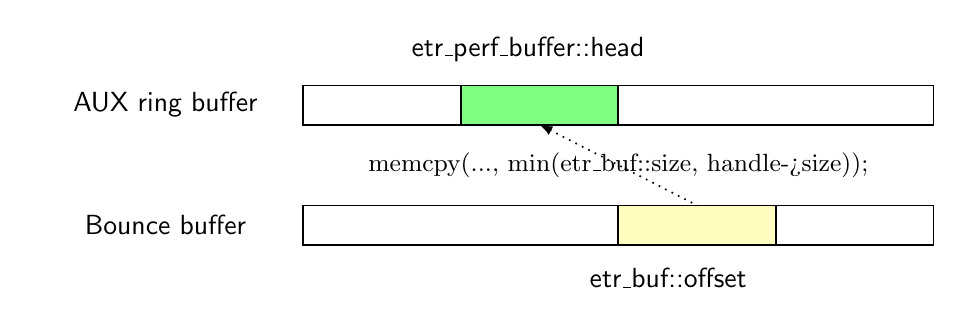
\begin{tikzpicture}[>=latex,font=\sffamily,semithick,scale=1.75]
	\node [minimum width=3.5cm,minimum height=.5cm,outer sep=0pt] at (0,0) (aux_rb1_txt) {AUX ring buffer};
	\node [minimum width=2cm,minimum height=.5cm,outer sep=0pt,draw=black,right=0cm of aux_rb1_txt] (aux_rb1_0) {};
	\node [minimum width=2cm,minimum height=.5cm,outer sep=0pt,draw=black,fill=green!50,right=0cm of aux_rb1_0] (aux_rb1_1) {};
	\node [minimum width=4cm,minimum height=.5cm,outer sep=0pt,draw=black,right=0cm of aux_rb1_1] (aux_rb1_2) {};

	\node [minimum width=3.5cm,minimum height=.5cm,outer sep=0pt,below=1cm of aux_rb1_txt] (bounce_buf1_txt) {Bounce buffer};
	\node [minimum width=4cm,minimum height=.5cm,outer sep=0pt,draw=black,right=0cm of bounce_buf1_txt] (boun_buf1_0) {};
	\node [minimum width=2cm,minimum height=.5cm,outer sep=0pt,draw=black,fill=yellow!25,right=0cm of boun_buf1_0] (boun_buf1_1) {};
	\node [minimum width=2cm,minimum height=.5cm,outer sep=0pt,draw=black,right=0cm of boun_buf1_1] (boun_buf1_2) {};

	\node [above left= .5em and -7em of aux_rb1_1] (lable1) {etr\_perf\_buffer::head};
	\node [below left= .5em and -5em of boun_buf1_1] (lable2) {etr\_buf::offset};
	\draw [<-,dotted] (aux_rb1_1.south) -- node[midway,yshift=0cm,font=\small] {memcpy(..., min(etr\_buf::size, handle->size)); } (boun_buf1_1.north);
\end{tikzpicture}
\par
\textbf{Figure 14: Syncing between bounce buffer and AUX ring buffer}
\end{center}

At the end of perf session, \code{etm\_free\_aux()} frees the data structures and the bounce buffer.

\subsection*{Some thoughts for further optimization}

As SG mode and CATU mode both support scatter-gather pages, the ETR driver can be improved to allow the hardware directly accessing AUX ring buffer; this can remove the redundant operations caused by the bounce buffer, the benefit is this can avoid the extra memory copying from the bounce buffer to the AUX buffer.

The second suggestion is to use normal memory mapping for the flat mode.  Rather than using the DMA mapping, the normal mapping can utilize the cache for boosting memory performance.  Though the memory size in flat mode is not so big with several megabytes, the performance improvement for memory copying with cacheable is still considerable.  And given this overload is caused by the tool itself, the optimization can avoid the noise for the profiling.

A potential minor improvement is to remove \code{etr\_perf\_buffer::head}, this field can be replaced by using \code{perf\_output\_handle::head} which contains the header for AUX ring buffer.

\end{document}
